\documentclass[tikz,border=5pt]{standalone}
\usepackage{pgfplots}
\usepackage{xcolor}
\pgfplotsset{compat=newest}

\pagecolor{white}

\begin{document}

    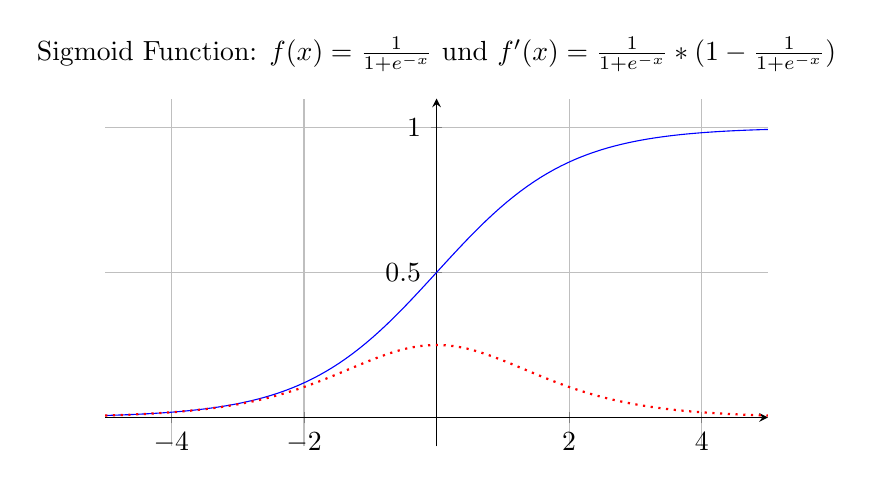
\begin{tikzpicture}
        \begin{axis} [
            axis lines=middle,
            samples=100,
            domain=-5:5,
            width=10cm,
            height=6cm,
            grid=both,
            ymin=-0.1,
            ymax=1.1,
            title={
                Sigmoid Function: 
                $f(x) = \frac{1}{1 + e^{-x}}$ 
                und 
                $f'(x) = {\frac{1}{1 + e^{-x}} * (1 - \frac{1}{1 + e^{-x}})}$},
        ]

        \addplot[blue, domain=-5:5] {1/(1+exp(-x))};
        \addplot[red, thick, dotted, domain=-5:5] {(1/(1+exp(-x))) * (1 - (1/(1+exp(-x))))};

        \end{axis}
    \end{tikzpicture}

\end{document}